%\todo{ALETHIA - first draft by 30/May}

%The search service provided by the Peer Manager (PM) was initially described in deliverable D4.2~\cite{D4.2}. In this deliverable we describe its evolution, by providing more details about the meta-data models that are related with the search and ranking techniques, as well as their implementations.
%
%\subsection{Mechanisms and algorithms}
%
%In order to select mechanisms and algorithms for implementing search in the PM we need to take into account existing approaches from the state of the art that can be used. For instance, there are many models and data structures that can be borrowed from the area of Information Retrieval (IR) as well as different matching techniques that can be used with different types of values. 
%%It is also important to define what is the atomic element (term) that will be used in the data and query representations.
%
%A logical view of the Search component is shown in Figure~\ref{fig:search_diagram}, and presents the internal mechanisms, called subcomponents, that are integrated within the PM to deal with different types of queries (i.e., constraints on values of different natures). 
%In what follows, these subcomponents are described in more details.
%
%In particular, the lower part of the figure shows two approaches that are used to deal with descriptions and names of peers. The upper part of the figure shows a subcomponent that builds on the other two to provide more flexible and heterogeneous language to access peer’s attributes as well as to provide additional operations. 

%\begin{figure}[htbp]
%\centering
%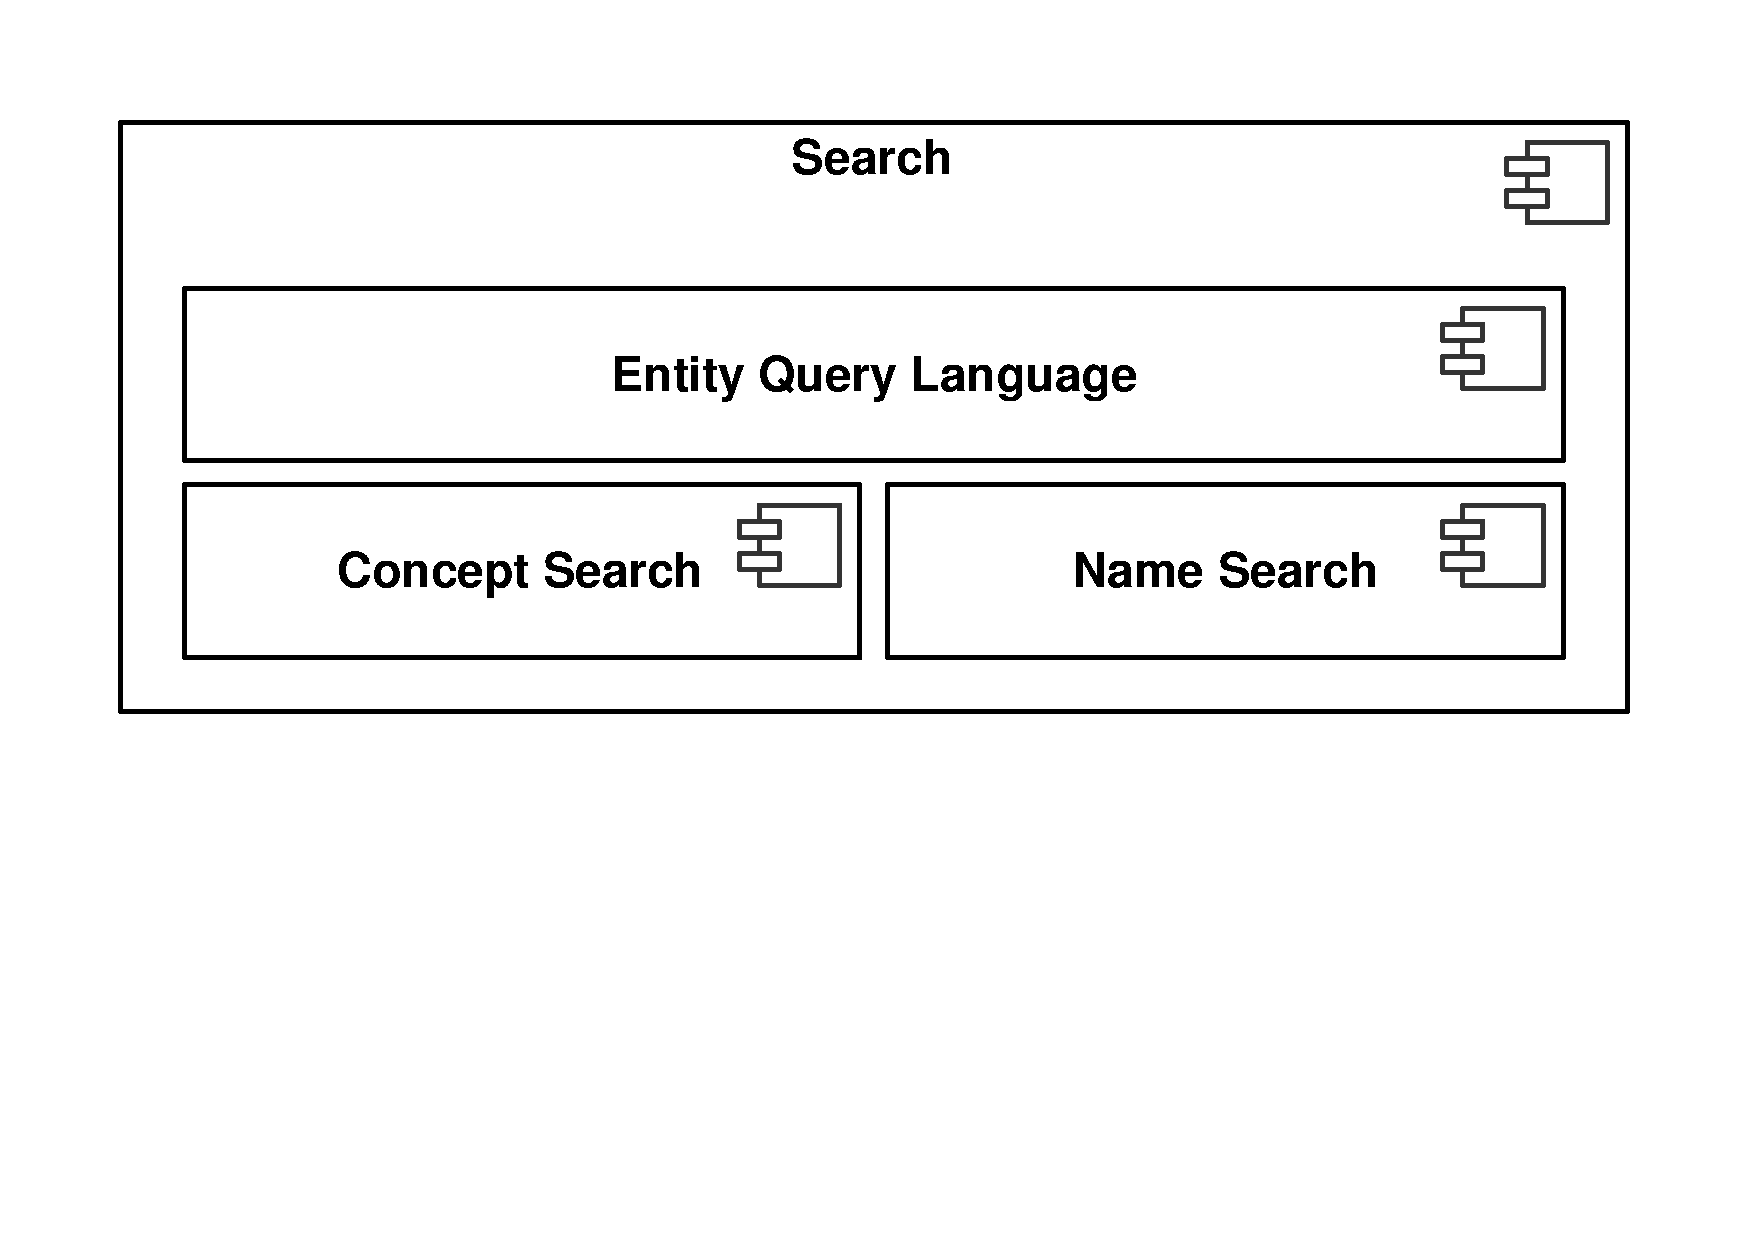
\includegraphics[width=0.65\textwidth]{figures/SearchComponentDiagram}
%\caption{Search Diagram}
%\label{fig:search_diagram}
%\end{figure}


%\subsubsection{Concept Search}
%\label{subsec:concept_search}
%Among existing IR models we can find the classical example of the vector space model that is used for computing query answers and relevance ranking. Among the different data structures used in IR systems, a widely used example for implementing efficient indexing and retrieval is the inverted index (also referred to as postings file or inverted file)\footnote{\url{http://en.wikipedia.org/wiki/Inverted_index}}. Next, we need to define the atomic element and the matching techniques to be used. 
%Many syntactic IR systems implement term matching by computing string similarity between words. Some examples of how term matching can be implemented are search for identical (possibly stemmed) words, words with common prefixes, words within a certain edit distance with a given word, or words that sound similarly (see~\cite{Manning:2008:IIR:1394399} for more details on existing syntactic search approaches). When trying to match peer's attributes with a search query in the PM, we consider also many problems that can negatively affect the quality of search results. In particular, we know that different words can have the same meaning (synonymy); the same word may have multiple meanings (polysemy); and the meaning of words can be different but still semantically related.

%In order to deal with these problems from syntactic information retrieval approaches, the PM uses Concept Search~\cite{Giunchiglia:2009fk} that extends the syntactic search with semantic search. In this approach, the retrieval models and data structures of syntactic search are reused. The main difference is given by the fact that concept search leverages on the core semantic data model of the PM and therefore concepts are used as terms instead of words. As a consequence, term matching is implemented by using semantic matching of concepts~\cite{Giunchiglia:2007ve}. On the other hand, when the semantic information is not available (for instance, when the concepts of a given set of words cannot be computed), words are used as terms and concept search falls back to the underlying syntactic search.

%Concept Search approach is used by the PM to implement concept based search on entity attributes (which include peer's attributes). The syntax of attribute based concept search queries is designed to be similar to the query syntax of Lucene\footnote{\url{http://lucene.apache.org/core/old_versioned_docs/versions/3_5_0/queryparsersyntax.html}}, a popular Java based open-source indexing and search library. The current implementation supports concept search on attribute values, e.g. the query \emph{``big restaurant''} among other results will also return entities with attributes containing phrase \emph{``huge steakhouse''}. Concept search is also implemented on top of attribute names, e.g. the entity with attribute \emph{``location:Trento''} will be returned as an answer to query \emph{``place:Trento''}. Atomic queries on attribute values and attribute names can be combined into more complex queries by using Boolean operators, e.g. \emph{``big restaurant AND location:Trento''}.

%\subsubsection{Name Search}
%\label{subsec:name_search}
%When dealing with peers that can be humans, it is important to account for the relevance of names, which are human readable identifiers that serve the purpose of distinguishing an entity from others. As a consequence, name search can be a common kind of search for named entities in an entity repository (EB) like the PM. The name search algorithm deals with the problem of finding all the possible candidate entities that have names equal or similar to a given name.
%
%Names are labels composed by a combination of words, numbers and symbols. They are different from other attributes because they play the role of keywords rather than been mapped to concepts from a knowledge base. As such, names can suffer from different types of variations. For example, they can have format variations (e.g., \emph{George Augusto Lombardi} vs. \emph{George A. Lombardi} vs. \emph{G. A. Lombardi} vs. \emph{Lombardi, George}), they can be translated (e.g., \emph{Trento} in Italian vs. \emph{Trient} in German vs. \emph{Trent} in English), they can be partially translated (e.g., \emph{University of} Trento vs.\emph{ Università di} Trento), or they can simply be misspelled (e.g., \emph{Fasuto} vs. \emph{Fausto} vs. \emph{Fuasot}). These name variations show the complexity with which a name search algorithm has to deal. Various syntactic search techniques can be used for implementing name search. 
%
%In the simplest case, name search is implemented by looking for exact matching of the provided name and the entity name. In order to address more complex cases, fuzzy search techniques can be employed. As a first step, names are tokenised and then tokens are compared. Jaccard~\cite{Bilenko:2003pd} similarity coefficient can be used for comparing the similarity\footnote{\url{http://en.wikipedia.org/wiki/Similarity_measure}} of token sets. Standard inverted index techniques can be used to efficiently implement this kind of search. Name tokens themselves can also be compared by using fuzzy search techniques. For instance, according to~\cite{Pollock:1984rr}, fewer errors usually occur at the beginning of names. Moreover, initials/abbreviations can be used instead of tokens representing parts of names. The two observations suggest that comparing prefixes of name tokens can be useful to improve the results of name search. Search for name tokens having the same prefix can be efficiently implemented both in the inverted index vocabulary and by using SQL like queries.\
%
%In the case of misspelled names, another efficient search technique that can be used is that of N-gram index. An n-gram is a continuous sequence of n characters for a given name token and the similarity between names is computed by counting number of co-occurring n-grams. In the current implementation we use trigrams (grams of length 3), which are extracted from each name token. Inverted index can be used to index names by using their trigrams, which allows for an efficient fuzzy name search. The pg\_trgm\footnote{\url{http://www.postgresql.org/docs/8.4/static/pgtrgm.html}}  module from PostgreSQL database management systems is used to implement trigram search on entity names in the current implementation. 
%%Note that PostgreSQL also supports other fuzzy search techniques in its fuzzystrmatch  module that allow computing similarities and distance between strings. Soundex and Metaphone are the methods used for matching similar-sounding names. Levenshtein edit distance metric is determined by the number of insertion, substitution and deletion of characters necessary to transform one name token into another. The edit distance is efficient for matching names containing typing errors.
%
%In the name search algorithm implemented by the PM, the techniques described above are applied in a sequential order until the entities with the matching names are found. Namely: 
%\begin{inparaenum}[(i)]
%\item Exact search is used as the most accurate results are provided by this technique; 
%\item Next, search with tokenized name is performed if no results are found by exact search; 
%\item Then, the prefix search is perfomed; and 
%\item Finally, the trigram search is used.
%\end{inparaenum}


%\subsubsection{Entity Query Language}
%\label{subsec:entity_query_language}

In order to combine different types of searches and to support additional search operations based on the relations between entities, an Entity Query Language (EQL) is used by the PM. EQL extends the low-level mechanisms, allowing more flexible access to the information of peers. EQL can be seen as a semantically enabled version of HQL\footnote{\url{http://docs.jboss.org/hibernate/core/3.3/reference/en/html/queryhql.html}} on entities, where HQL is an object-oriented query language similar to SQL. The Table~\ref{tab:hql_vs_eql} summarizes the main differences between HQL and EQL languages. 
\begin{table}[ht]
\small
\centering
\caption{HQL vs. EQL}
\begin{tabularx}{\linewidth}{|X|X|}
%\begin{longtabu} {|X|X|}
\hline
\multicolumn{1}{|c|}{\textbf{HQL}} & \multicolumn{1}{c|}{\textbf{EQL}} \\ 
\hline

\multicolumn{2}{|p{0.9\linewidth}|}{1. Entity types (in EQL) are used in place of Java classes/interfaces (in HQL).} \\
\hline
\textbf{Java Class} & \textbf{Entity Type (Concept)} \\
%\hline
\hdashline
\emph{from \textbf{eg.Cat} cat} & \emph{from \textbf{Cat} cat} \\
- returns all instances of the class eg.Cat & - returns all entities of the entity type Cat \\
- returns all instances of subclasses of eg.Cat & - returns all entities of more specific entity types \\
 & \textbf{Note:} in EQL syntax, the entity type is defined by using knowledge base concepts. Entity types with equivalent or more specific concepts are searched. \\
 \hline
 
\multicolumn{2}{|p{0.96\linewidth}|}{2. In EQL from clause, concept search queries can be used to pre-filter entities for specified types.} \\
\hline
Not supported & \textbf{Concept Search on attribute values} \\
%\hline
\hdashline
 & \emph{from Cat[\textbf{breed:longhair}] cat} \\
 & - returns all cats with bread attribute equivalent or more specific than longhair (e.g. Persian). \\
 & \textbf{Note:} Concept Search is described in Section~\ref{subsec:concept_search}. \\
 \hline

\multicolumn{2}{|p{0.9\linewidth}|}{3. Entity attributes (in EQL) are used in place of Java class properties (in HQL).} \\
\hline
\textbf{Java Class Property} & \textbf{Entity Attribute (Concept)} \\
%\hline
\hdashline
\emph{select \textbf{cat.name} from eg.Cat cat} & \emph{select \textbf{cat.name} from Cat cat} \\
- returns names of all the instances of eg.Cat & - returns names of all the entities of type Cat \\
 & \textbf{Note:} in EQL syntax, the entity attribute is defined by using knowledge base concepts. Entity attributes with equivalent or more specific concepts are searched. \\
\hline

\multicolumn{2}{|p{0.9\linewidth}|}{4. Meta-attributes.} \\
\hline
Not supported & \textbf{Meta-attributes} \\
%\hline
\hdashline
 & \emph{select cat.name, \textbf{m.veracity}} \\
 & \emph{from Cat cat join \textbf{cat.name.metadata} m} \\
 & - returns all cat names with corresponding veracity values. \\
 & \textbf{Note:} Only keywords \textbf{metadata}, \textbf{created}, and \textbf{modified} are allowed after an entity attribute name (e.g. \textbf{entity.attribute.metadata}), where created and modified are hard-coded meta-attributes and metadata is a structure for storing any additional user-created meta-attributes. \\
\hline
\end{tabularx}
%\end{longtabu}
\label{tab:hql_vs_eql}
\end{table}%



%\subsection{Implementation}
%
%The Peer Manager's implementation of its search service (search, matching and ranking services) uses Java in combination with Hibernate and Spring frameworks, a PostgreSQL database is used for storage of peers' information and profiles. The Peer Manager front-end uses NodeJs and exposes its basic search functionalities through a low level http API. In order to facilitate the interaction with other SmartSociety components (also in light of specific prototypes and DEMOs), the PM provides also a high level API that results in much more powerful and easy-to-use calls. Such calls leverage the full power of the Peer Manager and allow other components to abstract from internal details related to the PM's implementation. 
%
%It is important to note that the implementation of the underlying mechanisms at the core of the PM's search implementation represent previous knowledge/work of the University of Trento Knowdive research group, so its source code will not be made commonly available. However, the full source code of the high level API corresponding to the front-end implementation that is specific for SmartSociety will be made available as part of the project. In the rest of this section we provide more details on how to use the search service, which in turn is related with the implementation of the high level API. 

%\subsubsection{Search Service}
%%\todo{documentation of search service including syntax/examples of EQL}

\subsection{EQL Usage Example}

A more flexible access to search services require the specification of a search query using EQL language. The current implementation of the PM's search service supports a subset of HQL and new features can be added if (and when) needed. A simple example of an entity repository and examples of basic building blocks of EQL queries are shown in Fig.~\ref{fig:search_example} in order to introduce some of the search features that are currently implemented. 

%\todo{figure}
\begin{figure}[htbp]
\centering
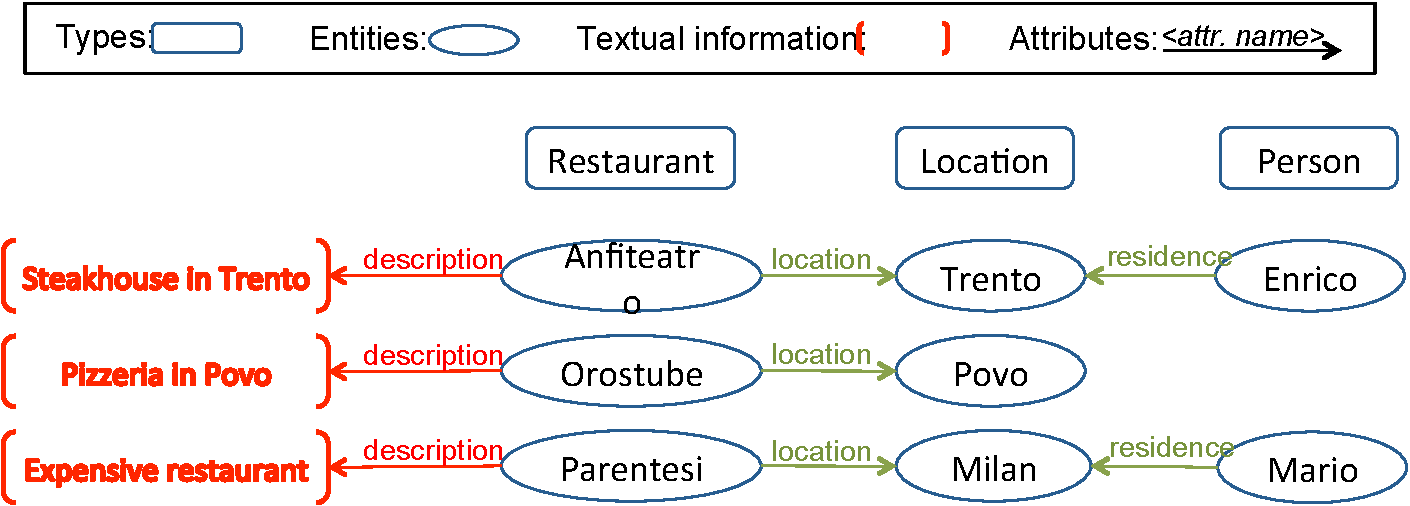
\includegraphics[width=0.90\textwidth]{figures/searchExample}
\caption{Example of simple entity repository}
\label{fig:search_example}
\end{figure}

The example entity repository has 3 entity types: \emph{Location}, \emph{Restaurant}, and \emph{Person}. Each entity type is instantiated by several entities. For instance, \emph{Trento}, \emph{Povo} and \emph{Milan} are names of entites of type \emph{Location}, \emph{Anfiteatro} is the name of a \emph{Restaurant} entity and \emph{Enrico} is the name of a \emph{Person} entity. Entities have different attributes, for instance, \emph{description} attribute of \emph{Location} entity contains textual information; while location attributes connect person and restaurant with locations correspondingly.

\paragraph{FROM clause.}
The simplest EQL query should contain at least the keyword \emph{from}, a type of entity, and an identifier for the resulting entities. For instance, in order to find all the restaurants stored in the entity repository, the query ``\texttt{FROM restaurant r}'' can be used.
%\begin{center}
%\begin{tabular}{l}
%\texttt{FROM restaurant r} \\
%\end{tabular}
%\end{center}
Note that there is no need to know the exact name of the entity type, concept search approach can also be used for matching entity types. For instance, in the case when there is a synonymy relationship between concepts \emph{restaurant} and \emph{bar} in the underlying knowledge base, the search to find all the restaurants can also be performed by using the query ``\texttt{FROM bar r}''.
%\begin{center}
%\begin{tabular}{l}
%\texttt{FROM bar r} \\
%\end{tabular}
%\end{center}

Another use of concept search query in \emph{from} clause can be to select a subset of all the entities for a given entity type. For instance, the following query finds only those restaurants that describe steakhouses:
\begin{center}
\begin{tabular}{l}
\texttt{FROM restaurant[description:steakhouse] r} \\
\end{tabular}
\end{center}
The query requires that descriptions of found restaurant entities contain complex concepts which are more specific than complex concept for `steakhouse', e.g. `steakhouse in Trento'.

\paragraph{SELECT clause.} 
The following query can be used to find descriptions and locations of all the restaurants. Which means to select attributes which are equivalent ore more specific than `description' and `location' of restaurant entities:
\begin{center}
\begin{tabular}{l}
\texttt{SELECT \textbf{restaurant1.description, restaurant1.location}} \\
\texttt{FROM restaurant \textbf{restaurant1}} \\
\end{tabular}
\end{center}
Note that also here there is no need to know the exact names for entity attributes. Equivalent or more general concepts can also be used. Moreover,
%For instance, we can search for related places with the query:
%\begin{center}
%\begin{tabular}{l}
%\texttt{SELECT restaurant1.description, \textbf{restaurant1.place}} \\
%\texttt{FROM restaurant restaurant1} \\
%\end{tabular}
%\end{center}
%Select 
the clause can also be used in combination with the selection of a subset of entities from a given type. For instance, find descriptions and related locations for all the steakhouses, i.e., select attributes which are equivalent ore more specific than `description' and `location' of restaurant entities with description containing complex concept (or concepts which are equivalent ore more specific than complex concept) `steakhouse':
\begin{center}
\begin{tabular}{l}
\texttt{SELECT restaurant1.description, \textbf{restaurant1.place}} \\ 
\texttt{FROM restaurant[\textbf{description:steakhouse}] restaurant1} \\
\end{tabular}
\end{center}

\paragraph{JOIN.}
Join on entities is probably the most important feature of EQL. For intance, the descriptions and location names for all the restaurants can be found with the following query:
\begin{center}
\begin{tabular}{l}
\texttt{SELECT restaurant1.description, location1.name} \\
\texttt{FROM \textbf{restaurant restaurant1 JOIN restaurant1.location location1}}
\end{tabular}
\end{center}
Note that an arbitrary number of joins is allowed with the following pattern:
\begin{center}
\begin{tabular}{l}
\texttt{... entity1 JOIN entity1.relationalAttribute entity2 ...}\\
\end{tabular}
\end{center}


\paragraph{GROUP BY, WHERE, and ORDER BY} clauses from HQL are supported also in EQL. Among them, the ORDER BY clause is of key importance because is the one that is used to implement the ranking of search results. For instance, to find the number of restaurants for each location and orders the results by location names (i.e., alphabetical order), we can use the query:
\begin{center}
\begin{tabular}{l}
\texttt{SELECT l.name, count(r)} \\
\texttt{FROM restaurant r join r.location l} \\
\texttt{GROUP BY l.name} \\
\texttt{ORDER BY l.name} \\
\end{tabular}
\end{center}
On the other hand, to order results by the number of restaurants on each location (i.e., numerical order), the following query can be used:
\begin{center}
\begin{tabular}{l}
\texttt{SELECT l.name, count(r)} \\
\texttt{FROM restaurant r join r.location l} \\
\texttt{GROUP BY l.name} \\
\texttt{ORDER BY count(r)} \\
\end{tabular}
\end{center}


\subsection{Limitations and Additional Notes}
It is also important to mention the \emph{current limitations}, which include:
\begin{enumerate}
\item \textbf{Joins:} Only inner join is supported, i.e., the keyword \emph{join} is used for specifying inner join.
\item \textbf{Nulls:} If an attribute name is selected, then only NOT NULL attribute values will be returned.

\begin{tabular}{ll}
\texttt{SELECT cat FROM Cat cat} & [all cats will be found] \\
\texttt{SELECT cat, cat.name FROM Cat cat} & [cats without names will be skipped] \\
\end{tabular}
\item \textbf{Aggregates:} Only simple aggregate functions on attributes are supported, e.g. count(cat).
\item \textbf{Dots:} As in HQL, dot-notation is used for accessing entity attributes. There are limitations on how dots are used. The first (and only the first) dot defines an attribute (e.g. cat.name). The second dot can be used only for accessing the meta-data (e.g. cat.name.metadata). Note, that it is not really a limitation because all the queries with two or more dots can be rewritten by using explicit joins, as it is shown below:

\begin{tabular}{p{0.45\textwidth}p{0.45\textwidth}}
\texttt{SELECT cat.mate.name} & [not supported] \\
\texttt{FROM Cat cat} & \\
 & \\
\texttt{SELECT mate.name}  & [equivalent query with explicit join] \\
\texttt{FROM Cat cat} & \\
\texttt{JOIN cat.mate mate} & \\
\end{tabular}
\end{enumerate}


The following are some \emph{additional notes} that are also important to take into account when interacting with the PM through EQL queries:
\begin{itemize}
\item If no attribute is specified in select or where clause, the entity id is used as a default attribute. For instance, 
``\texttt{SELECT cat FROM Cat cat}'' internally, will be translated to ``\texttt{SELECT cat.id FROM Cat cat}''

\item Specifying an alias (e.g. cat) is required. For instance, ``\texttt{FROM Cat cat}''

\item If concepts with multi-words are used for defining types or attributes, spaces between words should be replaced with underscore `\_'. For instance, ``\texttt{SELECT cat.first\_name FROM Cat cat}''.

\item Underscore `\_' can also be used for specifying correct concepts which should be used for attribute names and types. For instance, ``\texttt{SELECT cat.name\_123 FROM Cat\_321 cat}''.
\end{itemize}



%\subsubsection{Main Endpoints Documentation}
%\todo{The specification of the search APIs with an example will be added here for the final version of this document.}
%
%\begin{tabular}{llp{4cm}p{5cm}}
%\toprule
%Method & Api & Description & Example \\
%\midrule
%GET & /peers/search & Returns a set of profile of the peers that match with the characteristics specified in the input query & \\
%\bottomrule
%\end{tabular}











